\documentclass{beamer}
\usepackage{pgfpages}
\usepackage[backend=bibtex]{biblatex}
\usepackage{textpos}
\usepackage{multicol}
\setbeameroption{hide notes} % Only slides
%\setbeameroption{show only notes} % Only notes
%\setbeameroption{show notes on second screen=right} % Both
\bibliography{../../papers/references.bib}
\setbeamerfont{footnote}{size=\small}
%\AtEveryCitekey{\clearfield{title}}
\expandafter\def\expandafter\insertshorttitle\expandafter{%
   \insertshorttitle\hfill%
   \insertframenumber\,/\,\inserttotalframenumber}

%
% Choose how your presentation looks.
%
% For more themes, color themes and font themes, see:
% http://deic.uab.es/~iblanes/beamer_gallery/index_by_theme.html
%
\mode<presentation>
{
  \usetheme{Warsaw}      % or try Darmstadt, Madrid, Warsaw, ...
  \usecolortheme{default} % or try albatross, beaver, crane, ...
  \usefonttheme{default}  % or try serif, structurebold, ...
  \setbeamertemplate{navigation symbols}{}
  \setbeamertemplate{caption}[numbered]
  \usepackage{appendixnumberbeamer} %starts slide numbering over after \appendix
} 

\usepackage[english]{babel}
%\usepackage[utf8x]{inputenc} %Doesn't play well with biblatex
\usepackage{amssymb}
\usepackage{bm}
\usepackage{color}
\usepackage{graphicx}

\newcommand{\red}[1]{{\color{red}{#1}}}
\newcommand{\ket}[1]{\left| #1 \right>}
\newcommand{\bra}[1]{\left< #1 \right|}
\newcommand{\braket}[2]{\left< #1 | #2 \right>}
\newcommand{\ketbra}[2]{\left| #1 \right> \left< #2 \right|}
\newcommand{\expect}[1]{\left< #1 \right>}
\newcommand{\fpij}{f_p(r_{ij})}
\newcommand{\vpij}{v_p(r_{ij})}
\newcommand{\Opij}{\mathcal{O}_{ij}^p}
\newcommand{\fOpij}{\sum\limits_{i<j}\sum\limits_p \fpij\Opij}
\newcommand{\fqkl}{f_q(r_{kl})}
\newcommand{\Oqkl}{\mathcal{O}_{kl}^q}
\newcommand{\fOqkl}{\sum\limits_{k<l}\sum\limits_q \fqkl\Oqkl}
\newcommand{\fOqklip}{\sum\limits_{k<l,\mathrm{ip}}\sum\limits_q \fqkl\Oqkl}
\newcommand{\fOqklquad}{\sum_{\substack{k<l\\ij \ne kl}}\sum\limits_q \fqkl\Oqkl}
\newcommand{\f}[2]{f_{#1}(r_{#2})}
\renewcommand{\O}[2]{\mathcal{O}_{#2}^{#1}}
\newcommand{\fO}[2]{\sum\limits_{#1} f_{#1}(r_{#2})\mathcal{O}_{#2}^{#1}}
\renewcommand{\r}{\mathbf{r}}
\newcommand{\R}{\mathbf{R}}
\newcommand{\dt}{\Delta\tau}
\newcommand{\ti}{\bm{\tau}_i}
\newcommand{\tj}{\bm{\tau}_j}
\newcommand{\si}{\bm{\sigma}_i}
\newcommand{\sj}{\bm{\sigma}_j}
\newcommand{\sfont}{9}
\newcommand{\sspace}{10.2}

\title[Dissertation Defense]{{\large Dissertation Defense:}\\Improved Trial Wave Functions for Quantum Monte Carlo Calculations of Nuclear Systems and Their Applications}
\author[Cody L. Petrie]{Cody L. Petrie\\
Advisor: Kevin Schmidt}
\institute{Arizona State University}
%\date{}

\begin{document}

\begin{frame}
  \titlepage
\end{frame}

% Uncomment these lines for an automatically generated outline.
\begin{frame}{Outline}
  \tableofcontents
\end{frame}

% Commands to include a figure:
%\begin{figure}
%\includegraphics[width=\textwidth]{your-figure's-file-name}
%\caption{\label{fig:your-figure}Caption goes here.}
%\end{figure}

%\fontsize{\sfont}{\sspace}\selectfont
%\iffalse
\iftrue
\begin{frame}{Outline}
%Story: Why do we need to have a good trial wave function? Here are some options to improve the wave function. Here are the results we have gotten including some applications of the wave function.
\begin{itemize}
\only<1>{
   \item Background
   \begin{itemize}
      \item What is the problem we are trying to solve?
      \item Where are we applicable?
      \item Other methods
      \begin{itemize}
         \item HF - basis for other methods like AFDMC
         \item Basis set methods such as \ldots
         \item No-core shell model
         \item Coupled cluster
         \item self-consistent Green's function
      \end{itemize}
   \end{itemize}
   \item Methods to solve the nuclear problem and why we use QMC
   \begin{itemize}\fontsize{\sfont}{\sspace}\selectfont
      \item VMC
      \item DMC
      \item GFMC
      \begin{itemize}
         \item Excitations up to $^{12}$C
      \end{itemize}
      \item AFDMC
   \end{itemize}
}\only<2>{
   \item Trial wave function and why it's so important
   \begin{itemize}\fontsize{\sfont}{\sspace}\selectfont
      \item Slater Dets (and Pfaffians)
      \item Jastrow and linear correlations
      \begin{itemize}
         \item Results from previous papers showing the improvement
      \end{itemize}
      \item Quadratic correlations
      \begin{itemize}
         \item Results - show with jas $\rightarrow$ lin comparison as well
         \item Show the preliminary results we have with $\chi$EFT potentials as well.
         \item Performance scaling, both for xsede computers as well as linear vs. quadratic correlations.
      \end{itemize}
   \end{itemize}
   \item Other (future) correlations
   \begin{itemize}\fontsize{\sfont}{\sspace}\selectfont
      \item Exponential correlations
      \item Eigenvector discontinuity problem and square root matrix fix
      \item Preliminary results
   \end{itemize}
}\only<3>{
   \item Application to $\alpha$-clustering
   \begin{itemize}\fontsize{\sfont}{\sspace}\selectfont
      \item NS intro and why clustering is an interesting problem
      \begin{itemize}
         \item Clustering is often put in by hand, but we can do it {\it ab initio}.
      \end{itemize}
      \item Stefano's original results
      \item Results with quadratic correlations
   \end{itemize}
   \item Conclusion
   \item Extra Slides
   \begin{itemize}
      \item Add possible extra slides here when you think of them
   \end{itemize}
}
\end{itemize}
\end{frame}
\fi

\section{Motivation}
\begin{frame}{Nuclear Many Body Problem}
\vspace{-0.5cm}
\begin{equation*}
   \left<H\right> = \bra{\Psi}H\ket{\Psi} = \int\Psi^*(\bm{R})H\Psi(\bm{R}) d\bm{R}
\end{equation*}
\begin{equation*}
   H = \sum\limits_{i=1}^A \frac{\bm{p}^2}{2m} + \sum\limits_{i<j} v_{ij} + \sum\limits_{i<j<k} V_{ijk} + \ldots
\end{equation*}
\begin{figure}
   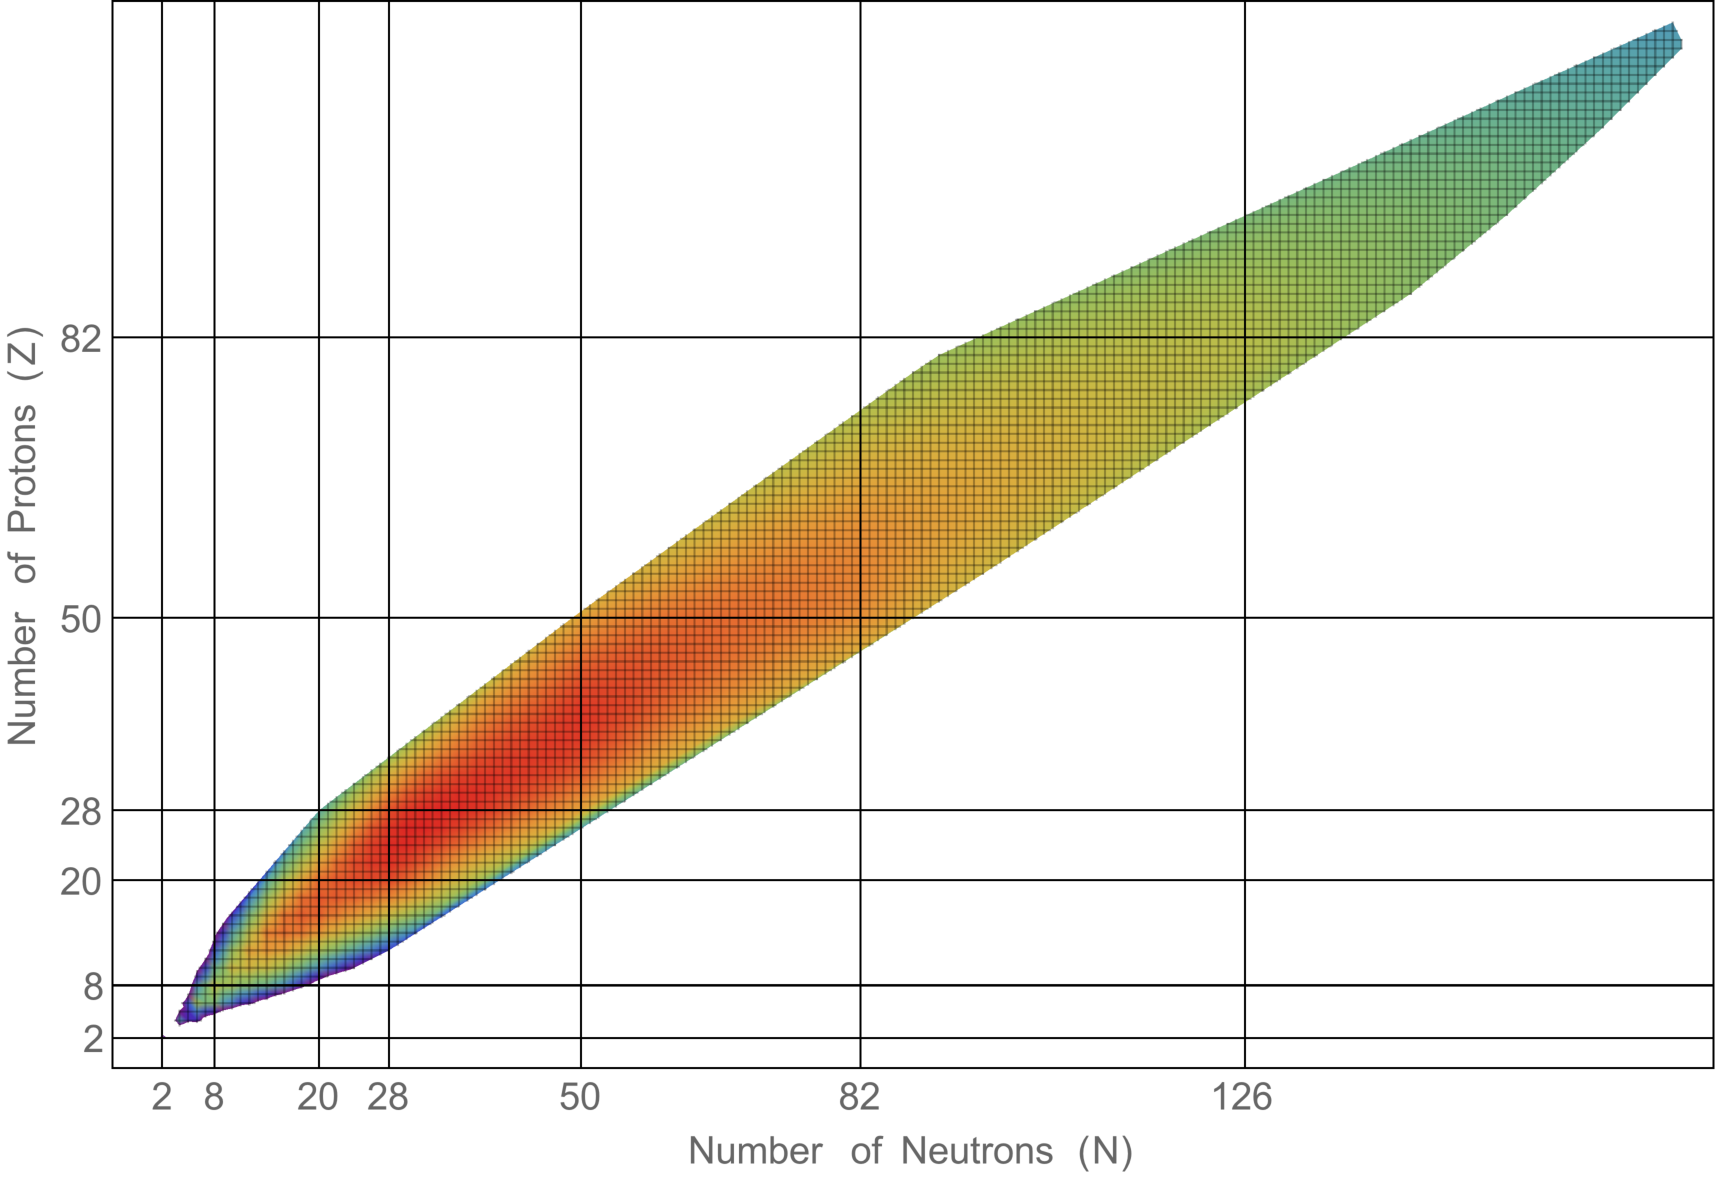
\includegraphics[width=0.65\textwidth]{../figures/tableofnuclides.pdf}
\end{figure}
\end{frame}
\note{Show on the chart up to where our method is applicable.}

\begin{frame}{Nuclear Many Body Methods}
\begin{itemize}
   \item There are a number of ways to solve this problem.
   \begin{itemize}
      \item Hartree-Fock
      \item Basis-set methods
      \begin{itemize}
         \item No-core shell model
         \item Coupled-cluster
         \item Self consistent Green's function method
      \end{itemize}
      \item Quantum Monte Carlo
      \begin{itemize}
         \item VMC
         \item GFMC
         \item AFDMC
      \end{itemize}
   \end{itemize}
\end{itemize}
\end{frame}

\section{Research}
\subsection{QMC Methods}
\begin{frame}{Variational Monte Carlo}
\begin{itemize}
   \item VMC starts with a trial wave function which includes variable parameters.
   \item The variational principle guarantees
   \begin{equation*}
      E_V = \frac{\int\psi_T^*(\R)H\psi_T(\R)d\R}{\int\psi_T^*(\R)\psi_T(\R)d\R} \ge E_0
   \end{equation*}
   \item We want this to look like this
   \begin{equation*}
      E_V = \int f(\R)P(\R) d\R \approx \frac{1}{N}\sum\limits_{n=1}^N f(\R_n)
   \end{equation*}
\end{itemize}
\end{frame}
\note{blah blah}

\begin{frame}{Variational Monte Carlo}
   \begin{equation*}
      E_V = \int P(\R)E_L(\R) d\R
   \end{equation*}
\begin{itemize}
   \item We can do that if we multiply by $\Psi_T(\R)\Psi_T^{-1}(\R)$.
%   \begin{align*}
%      P(\R) &= \frac{|\Psi_T(\R)|^2}{\int|\Psi_T(\R)|^2d\R} \\
%      E_L(\R) &= \Psi_T^{-1}(\R) H \Psi_T(\R)
%      E_L(\R) &= \frac{\Psi_T^*(\R) H \Psi_T(\R)}{\Psi_T^*(\R) \Psi_T(\R)}
%   \end{align*}
   \begin{equation*}
      P(\R) = \frac{|\Psi_T(\R)|^2}{\int|\Psi_T(\R)|^2d\R}, ~~~
%      E_L(\R) &= \Psi_T^{-1}(\R) H \Psi_T(\R)
      E_L(\R) = \frac{\Psi_T^*(\R) H \Psi_T(\R)}{\Psi_T^*(\R) \Psi_T(\R)}
   \end{equation*}
   \item Now using Monte Carlo integration we can write
   \begin{equation*}
      E_V \approx \frac{1}{N} \sum\limits_{n=1}^N E_L(\mathbf{R_n}),
   \end{equation*}
   where the $\R_n$ are samples from $P(\R)$.
\end{itemize}
\end{frame}

\begin{frame}{Variational Monte Carlo}
\begin{itemize}
   \item The statistical error in the energy is then given in the typical way
   \begin{equation*}
      \sigma_{E_V} = \sqrt{\frac{\left<E_L^2\right>-\left<E_L\right>^2}{N}} \approx \sqrt{\frac{\left(\frac{1}{N}\sum\limits_{n=1}^NE_L^2(\R_n)\right) - \left(\frac{1}{N}\sum\limits_{n=1}^NE_L(\R_n)\right)^2}{N-1}}
   \end{equation*}
   \item We can then vary the parameters in the trial wave function and calculate this until we minimize the energy or statistical error, since $E_V \ge E_0$.
\end{itemize}
\end{frame}

\begin{frame}{Diffusion Monte Carlo}
\begin{itemize}
   \item Diffusion Monte Carlo uses a Green's function to diffuse in imaginary time to estimate the ground state energy and wave function based on a trial wave function.
   \begin{equation*}
      H\Psi = i\hbar\frac{d\Psi}{dt} ~ \xrightarrow{\tau=it/\hbar} ~ H\Psi = -\frac{d\Psi}{d\tau}
   \end{equation*}
   Using separation of variables we can write
   \begin{equation*}
      \Psi(\R,\tau) = \sum\limits_{n=0}^{\infty} c_n\phi_n(\R) e^{-\tau(E_n-E_0)}
   \end{equation*}
   \item The long imaginary time limit of this goes to the ground state.
   \begin{equation*}
      \lim\limits_{\tau\rightarrow\infty} \Psi(\R,\tau) = c_0\phi_0(\R)
   \end{equation*}
\end{itemize}
\end{frame}
\note{We start DMC from the minimized $\psi_T$ and configurations from VMC.}

\begin{frame}{Diffusion Monte Carlo}
\begin{itemize}
   \item The propagated wave function can be written
   \begin{equation*}
      \braket{\R'}{\Psi_T(\tau)} = \int d\R \bra{\R'}e^{-(H-E_0)\tau}\ket{\R}\braket{\R}{\Psi_T(0)}
   \end{equation*}
   \item Now we use $e^{-H\tau}=e^{-V\tau/2}e^{-T\tau}e^{-V\tau/2}+\mathcal{O}(\tau^3)$ and break up the propagator into small time steps $\dt = \tau/N$.
   \begin{equation*}
      \braket{\R_N}{\Psi_T(\tau)} = \int d\R_1 \ldots d\R_N \left[\prod\limits_{i=1}^N G(\R_i,\R_{i-1},\Delta\tau)\right] \braket{\R_0}{\Psi_T(0)}
   \end{equation*}
   \begin{equation*}
      G(\R',\R,\Delta\tau) = \bra{\R'}e^{-(H-E_0)\Delta\tau}\ket{\R}
   \end{equation*}
\end{itemize}
\end{frame}

\begin{frame}{Diffusion Monte Carlo}
\begin{itemize}
   \item In the small $\dt$ limit this propagator can be split up with the kinetic term being used to diffuse the walkers along a random path.
   \begin{equation*}
      \bra{\R'}e^{-T\Delta \tau}\ket{\R} = \left(\frac{m}{2\pi\hbar^2\Delta\tau}\right)^{3A/2}e^{-m(\R'-\R)^2/2\hbar^2\Delta\tau}
   \end{equation*}
   \item The potential term can then be used as a weight in a branching algorithm.
   \begin{equation*}
      w(\R') = e^{-\left(V\left(\R'\right)+V\left(\R\right)-2E_0\right)\Delta\tau/2}%\bra{\R'}e^{-(V-E_0)\Delta\tau}\ket{\R}
   \end{equation*}
   \item Importance sampling improves the variance of the sampling and can be included with
   \begin{equation*}
      G(\R',\R,\Delta\tau) \rightarrow G(\R',\R,\Delta\tau)\frac{\braket{\R}{\Psi_I}}{\braket{\R'}{\Psi_I}}
   \end{equation*}
\end{itemize}
\end{frame}

\begin{frame}{Diffusion Monte Carlo}
Branching: Each walker can be deleted or multiply. The number of walkers that continues is equal to $\mathrm{int}\left(w(\R')+\xi\right)$, where $\xi$ is a uniform random number from $[0,1]$.
\begin{columns}
\begin{column}{0.4\textwidth}
\begin{figure}
   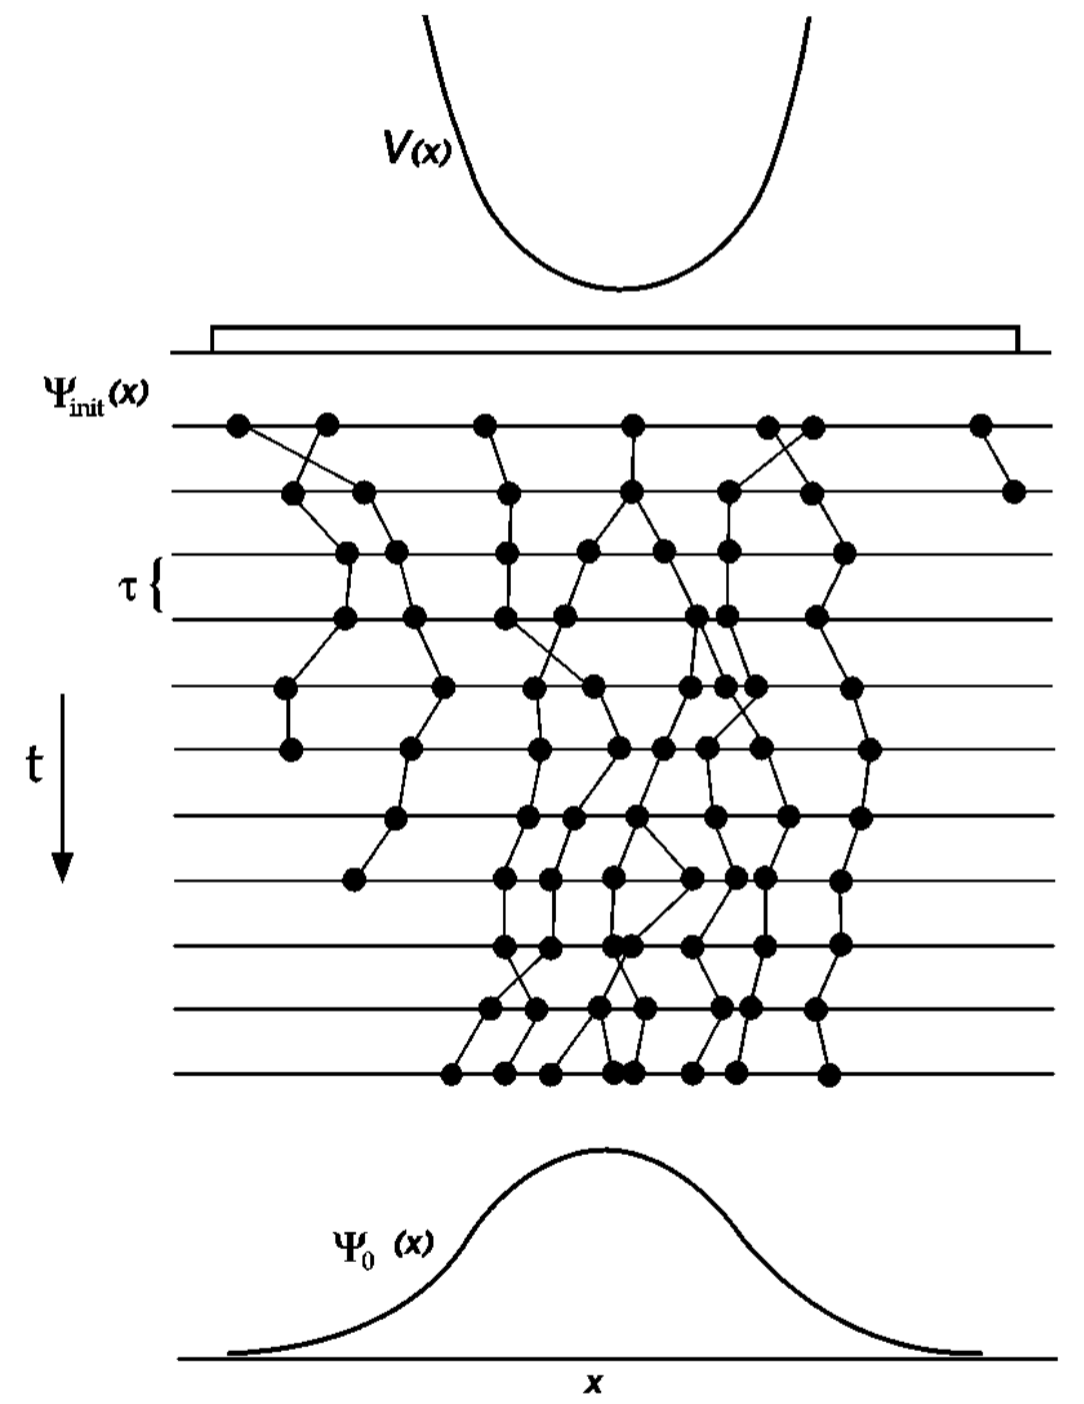
\includegraphics[width=0.9\textwidth]{../figures/branching.png}
\end{figure}
\end{column}
\begin{column}{0.7\textwidth}
   {\color{blue}{Figure:}} Reprinted from W.M.C. Foulkes et al. \textit{Rev. Mod. Phys.,} 73:33-83, 2001.
\end{column}
\end{columns}
\end{frame}

\begin{frame}{Estimating Expectation Values}
We want to solve something like this
\begin{equation*}
   \left<\mathcal{O}\right> = \frac{\bra{\Psi(\tau)}\mathcal{O}\ket{\Psi(\tau)}}{\braket{\Psi(\tau)}{\Psi(\tau)}}.
\end{equation*}
In practice a linear extrapolation is used because $\mathcal{O}\Psi(\tau)$ is hard.
\begin{equation*}
   \left<\mathcal{O}\right> \approx 2\left<\mathcal{O}\right>_\text{mixed} - \left<\mathcal{O}\right>_\text{VMC}
\end{equation*}
\begin{equation*}
   \left<\mathcal{O}\right>_\text{mixed} = \frac{\bra{\Psi(\tau)}\mathcal{O}\ket{\Psi_T}}{\braket{\Psi(\tau)}{\Psi_T}},
   ~~~~
   \left<\mathcal{O}\right>_\text{VMC} = \frac{\bra{\Psi_T}\mathcal{O}\ket{\Psi_T}}{\braket{\Psi_T}{\Psi_T}}
\end{equation*}
In the large $\tau$ limit when $\left[\mathcal{O},H\right]$=0
\begin{equation*}
   \lim\limits_{\tau\rightarrow\infty}\left<\mathcal{O}\right>_\text{mixed} = \left<\mathcal{O}\right>
\end{equation*}
\end{frame}

\begin{frame}{Estimating Error}
Our energy estimates are correlated and so we estimate error using block averaging
\begin{figure}
   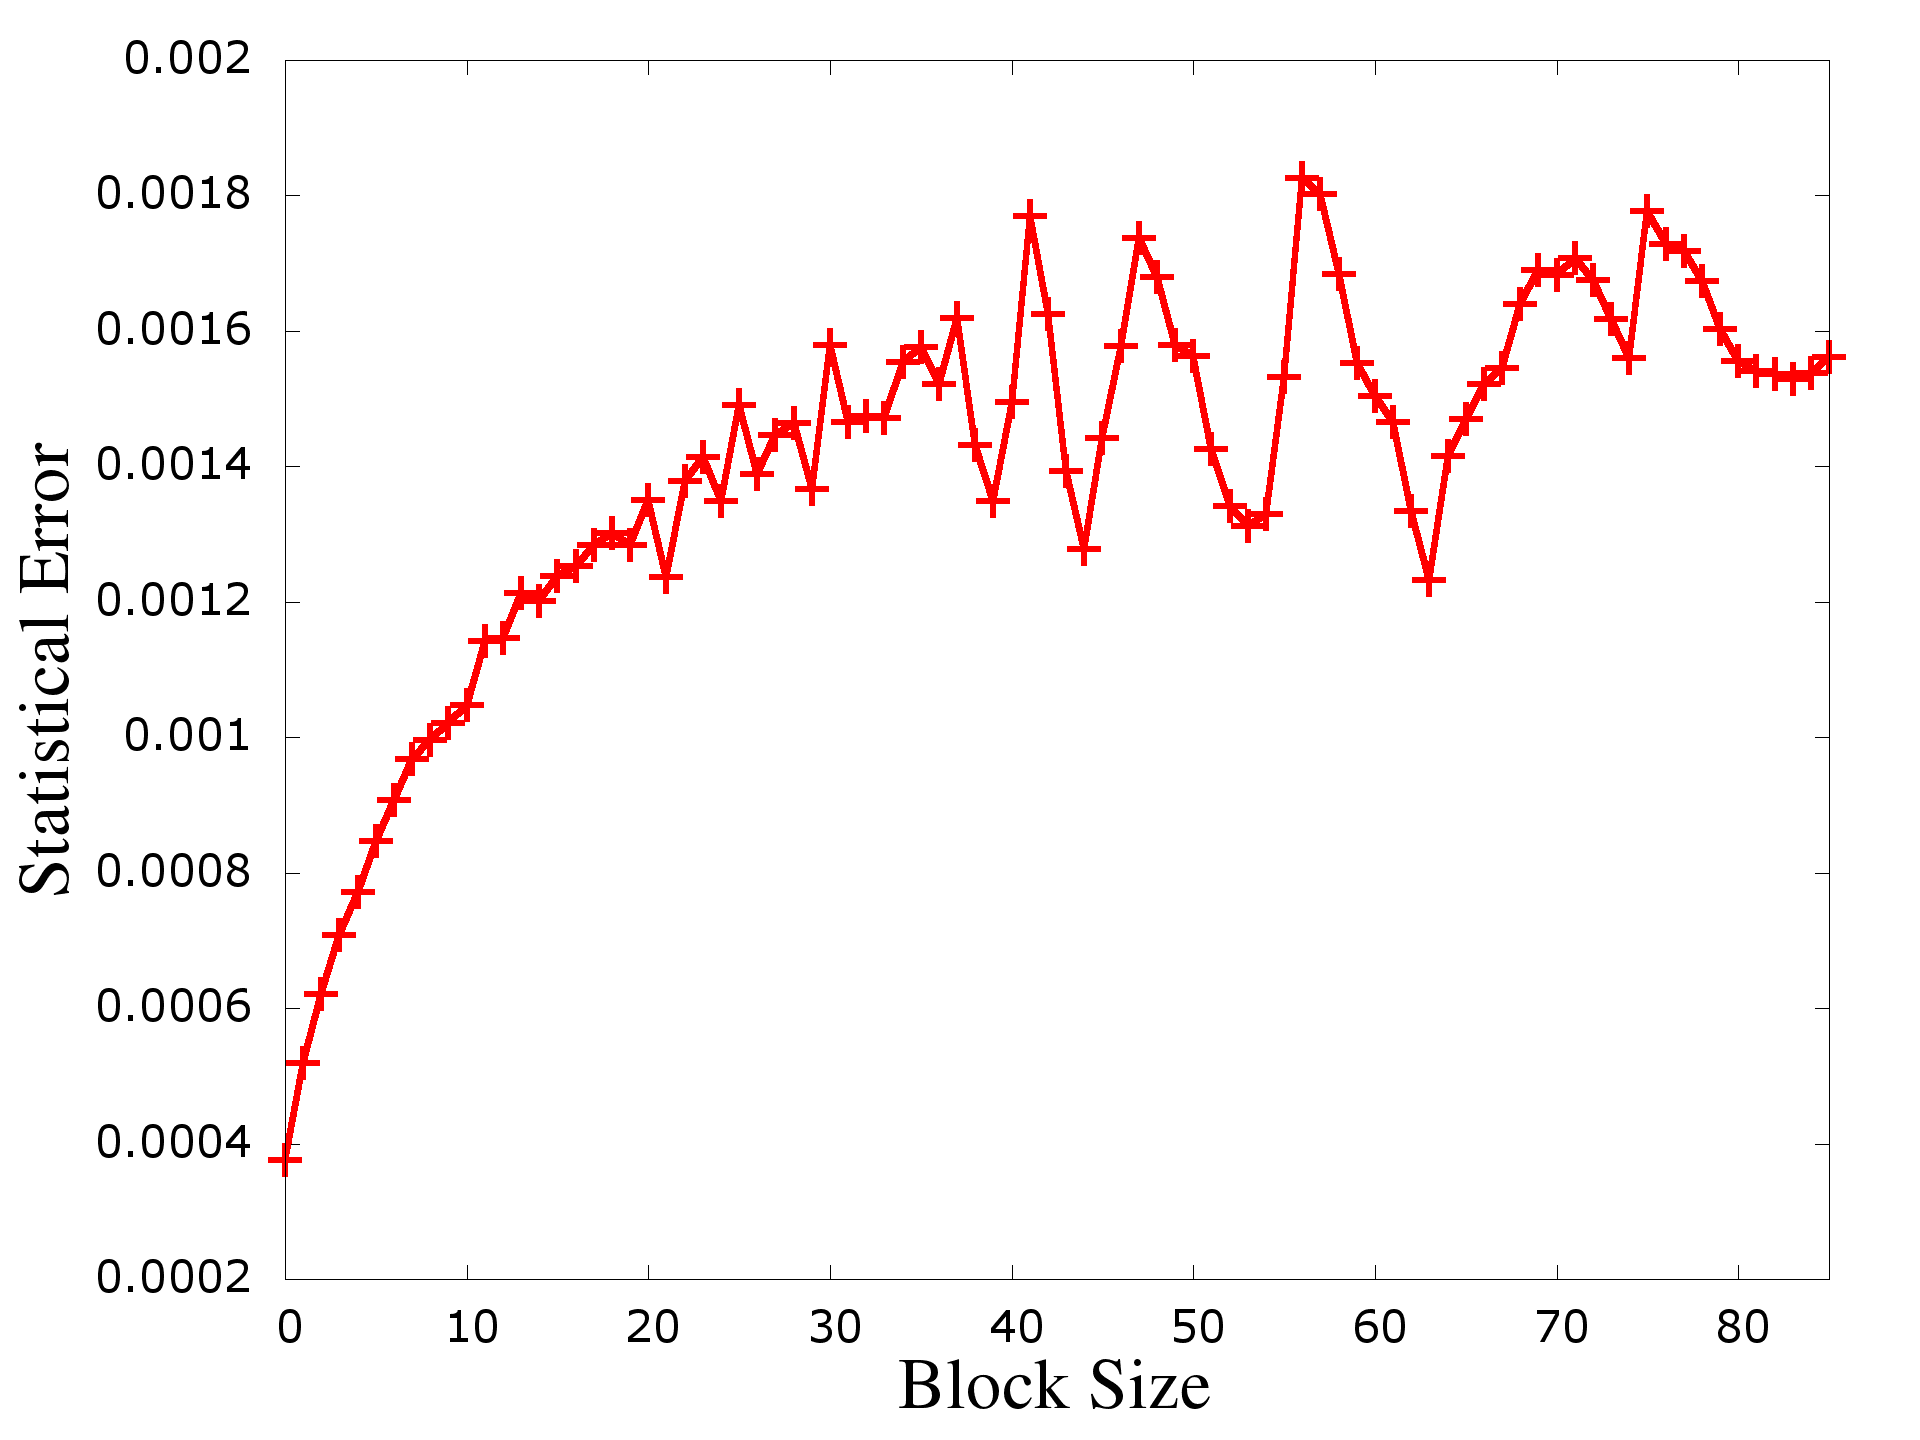
\includegraphics[width=0.77\textwidth]{../figures/blockaverage.png}
\end{figure}
\end{frame}

\begin{frame}{Green's Function Monte Carlo}
\begin{itemize}
   \item GFMC follows DMC exactly for the spatial integrals, but performs the sums of $2^A$ spin and $\frac{A!}{Z!(A-Z)!}$ isospin states, for $A$ nucleons with $Z$ protons explicitly.
\end{itemize}
\begin{figure}
   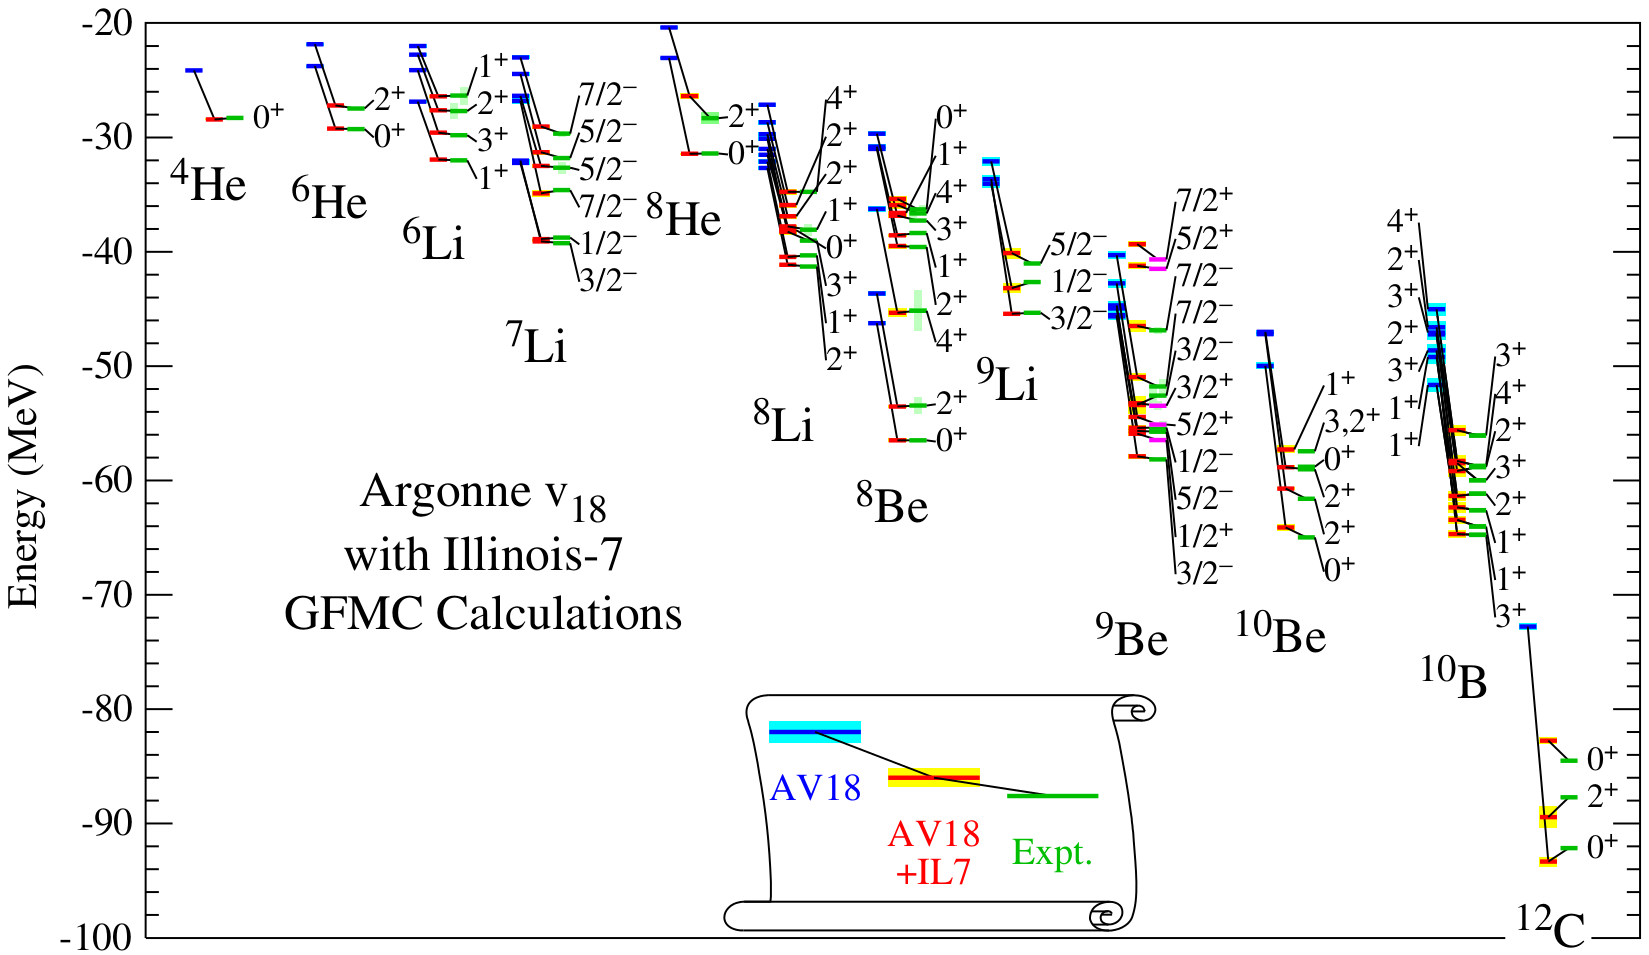
\includegraphics[width=0.85\textwidth]{../figures/gfmc_energies.png}
\end{figure}
\end{frame}

\begin{frame}{Auxiliary Field Diffusion Monte Carlo - Spin Sampling}
\begin{itemize}
   \item AFDMC samples auxiliary fields to rotate the spins/isospins of the walkers.
   \item The spin/isospin dependent part of the potential is what is used in the spin/isospin dependent part of the propagator.
   \begin{equation*}
      G_{SD}(R'S',RS,\dt) = \bra {R'S'}e^{-V_{SD}\dt} \ket{RS}
   \end{equation*}
   \begin{equation*}
      V_{SD} = \sum\limits_{p=2}^6\sum\limits_{i<j}v_p(r_{ij})\Opij
   \end{equation*}
   \item For $v_6$, a truncation of the phenomenological Argonne $v_{18}$ potential, the operators are $\si\cdot\sj$, $\ti\cdot\tj$, $\si\cdot\sj \ti\cdot\tj$, $S_{ij}$ and $S_{ij} \ti\cdot\tj$, where $S_{ij} = 3\si\cdot\hat{r}_{ij}\sj\cdot\hat{r}_{ij}-\si\cdot\sj$
\end{itemize}
\end{frame}

\begin{frame}{Auxiliary Field Diffusion Monte Carlo - Spin Sampling}
\begin{itemize}
   \item To avoid explicitly doing the $2^A\frac{A!}{Z!(A-Z)!}$ sums over the spin-isospin states AFDMC writes the spin-isospin dependent propagator in terms of squared single particle operators.
   \item The spin-isospin dependent operators
   \begin{equation*}
      e^{-V_{SD}\dt}
   \end{equation*}
   is sampled by using the Hubbard-Stratanovich transformation.
   \begin{equation*}
      e^{-\frac{1}{2}\lambda O^2} = \frac{1}{\sqrt{2\pi}} \int dx e^{-\frac{x^2}{2} + \sqrt{-\lambda}xO}
   \end{equation*}
\end{itemize}
\end{frame}
\note{This process will come up again when talking about the exponential correlations.}

\begin{frame}{Auxiliary Field Diffusion Monte Carlo - Spin Sampling}
\begin{itemize}
   \item The potential can be written in terms of matrices that are made of the $v_p(r_{ij})$, are symmetric, and 0 if $i=j$.
   \begin{equation*}
      V_{SD} = \frac{1}{2}\sum\limits_{i\alpha j\beta} \sigma_{i\alpha}A^{\sigma}_{i\alpha j\beta}\sigma_{j\beta}
      + \frac{1}{2}\sum\limits_{i\alpha j\beta} \sigma_{i\alpha}A^{\sigma\tau}_{i\alpha j\beta}\sigma_{j\beta}\ti\cdot\tj
      + \frac{1}{2}\sum\limits_{ij} A^{\tau}_{ij}\ti\cdot\tj
   \end{equation*}
   \item We can construct these matrices and then solve for their eigenvalues and eigenvectors.
\begin{align*}
   &\sum\limits_{j\beta} A^{\sigma}_{i\alpha j\beta}\psi^{\sigma}_{nj\beta} = \lambda^{\sigma}_n\psi^{\sigma}_{ni\alpha} \\
   &\sum\limits_{j\beta} A^{\sigma\tau}_{i\alpha j\beta}\psi^{\sigma\tau}_{n j\beta} = \lambda^{\sigma\tau}_n\psi^{\sigma\tau}_{ni\alpha} \\
   &\sum\limits_{j} A^{\tau}_{ij}\psi^{\tau}_{n,j} = \lambda^{\tau}_n\psi^{\tau}_{ni}
\end{align*}
\end{itemize}
\end{frame}

\begin{frame}{Auxiliary Field Diffusion Monte Carlo - Spin Sampling}
\begin{itemize}
   \item The potential can then be written in terms of the square of new single particle operators.
   \begin{equation*}
      V_{SD} = \frac{1}{2}\sum\limits_{n=1}^{3A} \left(O_{n}^{\sigma}\right)^2 \lambda_n^{\sigma}
      + \frac{1}{2}\sum\limits_{\alpha=1}^{3}\sum\limits_{n=1}^{3A} \left(O_{n\alpha}^{\sigma\tau}\right)^2 \lambda_n^{\sigma\tau}
       + \frac{1}{2}\sum\limits_{\alpha=1}^{3}\sum\limits_{n=1}^{A} \left(O_{n\alpha}^{\tau}\right)^2 \lambda_n^{\tau}
   \end{equation*}
   \begin{equation*}
   \begin{split}
      O_{n}^{\sigma} &= \sum\limits_{j\beta} \sigma_{j\beta}\psi_{nj\beta}^{\sigma} \\
      O_{n\alpha}^{\sigma\tau} &= \sum\limits_{j\beta} \tau_{j\alpha}\sigma_{j\beta}\psi_{nj\beta}^{\sigma\tau} \\
      O_{n\alpha}^{\tau} &= \sum\limits_{j} \tau_{j\alpha}\psi_{nj}^{\tau}
   \end{split}
   \end{equation*}
\end{itemize}
\end{frame}

\begin{frame}{Auxiliary Field Diffusion Monte Carlo - Spin Sampling}
\begin{itemize}
   \item Since we have squared single particle operators in the propagator we can now rewrite the propagator in terms of the Hubbard-Stratanovich transformation.
   \begin{equation*}
      e^{-\frac{1}{2}\lambda O^2} = \frac{1}{\sqrt{2\pi}} \int dx e^{-\frac{x^2}{2} + \sqrt{-\lambda}xO}
   \end{equation*}
   \item Since we have 15A operators ($3A$ for $O_{n}^{\sigma}$, $9A$ for $O_{n\alpha}^{\sigma\tau}$, and $3A$ for $O_{n\alpha}^{\tau}$), the spin-isospin dependent part of the propagator becomes
   \begin{equation*}
      G_{SD}(R'S',RS,\dt) = \prod\limits_{n=1}^{15A}\frac{1}{\sqrt{2\pi}}\int dx_n e^{-\frac{x_n^2}{2}}e^{\sqrt{-\lambda_n\dt} x_nO_n}.
   \end{equation*}
\end{itemize}
\end{frame}

\begin{frame}{Hamiltonian}
%Meson+phenomonological terms with picture of scattering and maybe pion exchange
%$\chi$EFT with picture of something related to that...
\begin{columns}
\begin{column}{0.5\textwidth}
\begin{figure}
   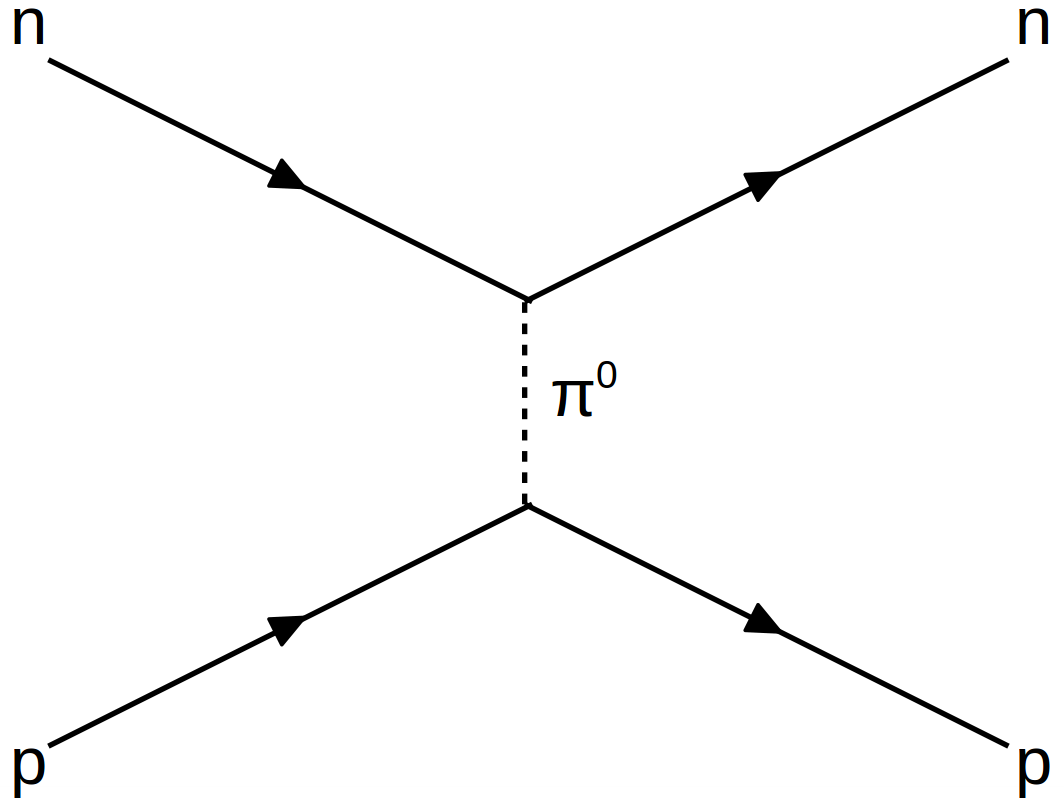
\includegraphics[width=0.75\textwidth]{../figures/pionexchange.png}
\end{figure}
\end{column}
\begin{column}{0.5\textwidth}
   Based on meson exchange
   \begin{itemize}
      \item Argonne $v_{18}$ (NN)
      \item CD-Bonn (NN)
      \item Urbana UIX (NNN)
      \item Illinois (NNN)
   \end{itemize}
\end{column}
\end{columns}
\begin{columns}
\begin{column}{0.5\textwidth}
\begin{figure}
   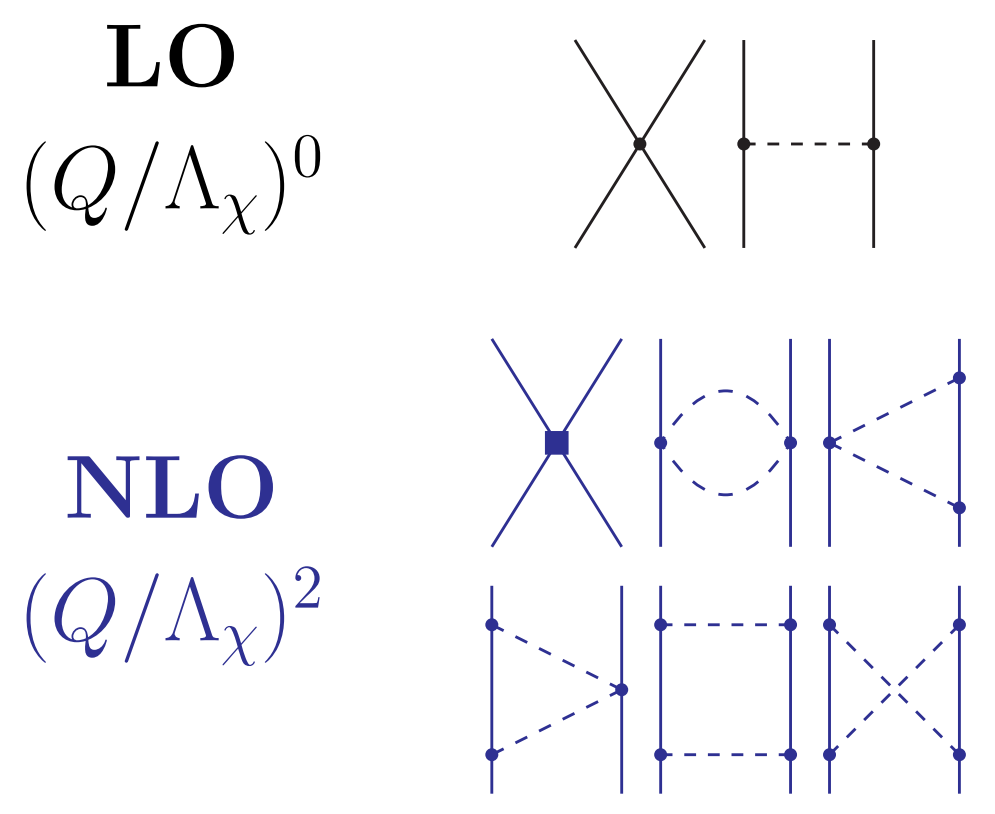
\includegraphics[width=0.75\textwidth]{../figures/chpt.png}
\end{figure}
\end{column}
\begin{column}{0.5\textwidth}
   Based on $\chi$EFT expansion in momentum (up to N2LO)
   {\\ \tiny Figure from R. Machleidt and D.R. Entem, {\it Chiral effective field theory and nuclear forces}, Phys. Rep. {\bf 503}, 1 (2011)}
\end{column}
\end{columns}
\end{frame}

\begin{frame}{Hamilatonian - Argonne $v6'$ (AV6$'$)}
\begin{itemize}
   \item For this work I have used the NN AV6$'$ potential with no 3N interaction, though I will be showing some preliminary results with the $\chi$EFT NN and 3N potentials up to N2LO.
   \item First 6 operators of the AV18 potential
   \begin{equation*}
      v_{ij} = \sum\limits_{p=1}^6 v_p(\r_{ij})\mathcal{O}^p_{ij}
   \end{equation*}
   \begin{equation*}
      \mathcal{O}^p_{ij} = 1,~\ti\cdot\tj,~\si\cdot\sj,~\si\cdot\sj\ti\cdot\tj,~S_{ij},~S_{ij}\ti\cdot\tj
   \end{equation*}
   \begin{equation*}
      S_{ij} = 3\si\cdot\hat{r}_{ij}\sj\cdot\hat{r}_{ij}-\si\cdot\sj
   \end{equation*}
\end{itemize}
\end{frame}

\subsection{Trial Wave Function}
\begin{frame}{Slater Determinant}
\begin{itemize}
   \item Properties:
   \begin{itemize}
      \item Antisymmetric
      \item Cluster Decomposable \\ $\ket{A+B} = \ket{A}\ket{B}$
   \end{itemize}
   \begin{textblock*}{\textwidth}(4.5cm,-6.1cm) % {block width} (coords)
      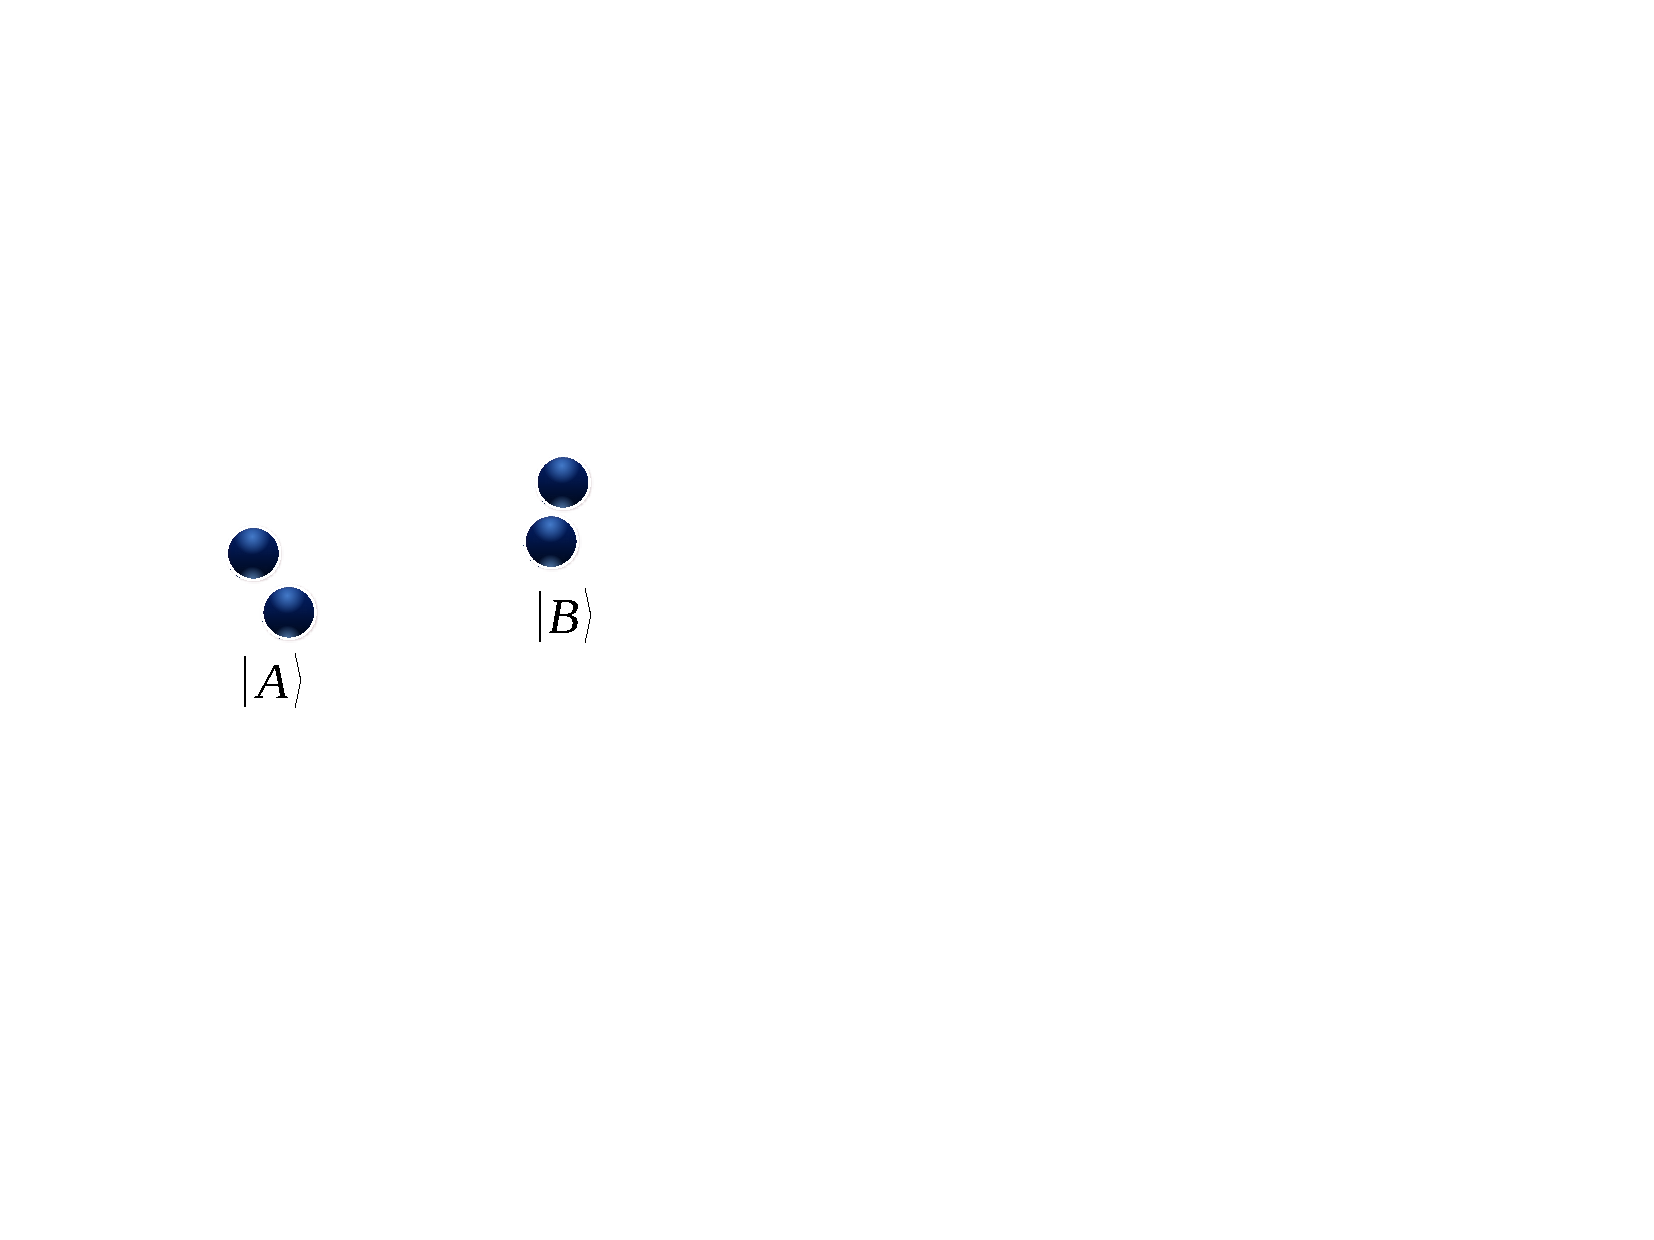
\includegraphics[width=14.6cm]{../figures/cluster.pdf}
   \end{textblock*}
   \item The simplest wave function for a many-fermion system obeying these properties is a Slater determinant where $\phi_i(\mathbf{r}_i,s_i)$ are single particle nucleon states.
   \begin{equation*}
      \psi_{T} = \braket{RS}{\phi}= \mathcal{A} \prod\limits_{i=1}^A \phi_i(\mathbf{r}_i,s_i) = \frac{1}{A!} \mathrm{det}~\phi_i(\mathbf{r}_i,s_i)
   \end{equation*}
   \item Short range correlations need to be put in by hand via Jastrow-like correlations.
   \begin{equation*}
      \ket{\psi_T} = \prod\limits_{i<j}f(r_{ij}) \ket{\phi}.
   \end{equation*}
\end{itemize}
\end{frame}

\begin{frame}{Spin Dependent Correlations}
\begin{itemize}
   \item Two spin dependent wave functions that obey these two properties are the exponentially correlated and symmetrized product wave functions, where $\Opij$ are the AV6 operators, $\si\cdot\sj$, $\ti\cdot\tj$,     $\si\cdot\sj \ti\cdot\tj$, $S_{ij}$ and $S_{ij} \ti\cdot\tj$, where $S_{ij}     = 3\si\cdot\hat{r}_{ij}\sj\cdot\hat{r}_{ij}-\si\cdot\sj$.
   \begin{equation*}
      \ket{\psi_T} = \left[\prod\limits_{i<j}f_c(r_{ij})\right] e^{\sum\limits_{i<j}\sum\limits_p\fpij\Opij} \ket{\phi}
   \end{equation*}
   \begin{equation*}
      \ket{\psi_T} = \left[\prod\limits_{i<j}f_c(r_{ij})\right] \mathcal{S}\prod\limits_{i<j}\left(1+\sum\limits_p\fpij\Opij\right) \ket{\phi}
   \end{equation*}
   \item These two wave functions are the same up to second order except for  commutator terms.
\end{itemize}
\end{frame}

\begin{frame}{Expand to Linear Correlations}
\begin{itemize}
   \item Because of the cost for larger systems in 2007 they only included Jastrow correlations.
   \begin{equation*}
      \ket{\psi_T} = \left[\prod\limits_{i<j}f_c(r_{ij})\right]\ket{\phi}
   \end{equation*}
   {\tiny S. Gandolfi et al. \textit{Phys. Rev. Lett.,} \textbf{99}, 022507, 2007.}
   \item By 2014 they added spin-isospin correlations to improve overlap with tensor. This is a truncated expansion of either full wave function from before.
   \begin{equation*}
      \ket{\psi_T} = \left[\prod\limits_{i<j}f_c(r_{ij})\right] \left(1+\sum\limits_{i<j}\sum\limits_p\fpij\Opij\right) \ket{\phi}
   \end{equation*}
   {\tiny S. Gandolfi et al. \textit{Phys. Rev. C.,} \textbf{90}, 061306(R), 2014.}
\end{itemize}
\end{frame}

\begin{frame}{Compare Jastrow to Jastrow+Linear}
\begin{figure}[h]
   \centering
   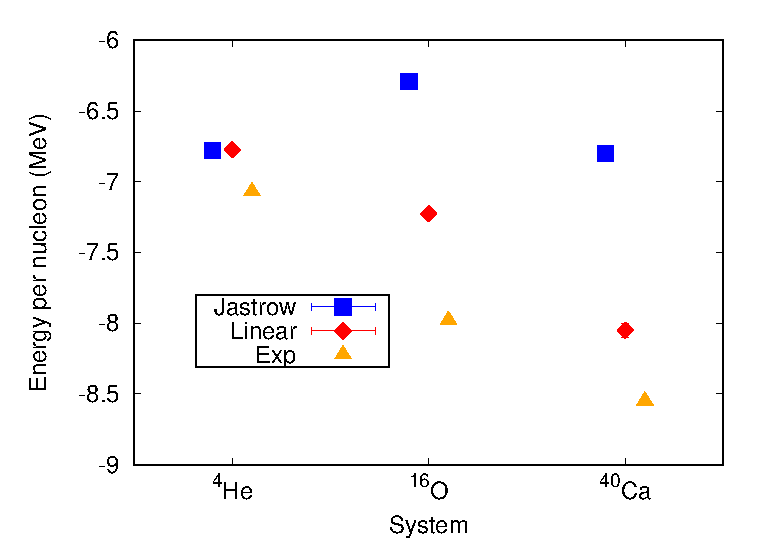
\includegraphics[width=0.85\textwidth]{../figures/energy_jaslin.eps}
\end{figure}
\vspace{-0.5cm}
{\tiny Data taken from each paper respectively.}
\end{frame}

\begin{frame}{Symmetrized Product Wave Function}
\begin{itemize}
   \item The logical next step was to keep more terms in the expansion.
   \begin{equation*}
   \begin{split}
      \ket{\psi_T} = \Bigg[\prod\limits_{i<j}&f_c(r_{ij})\Bigg] \Bigg[1+\fOpij \\
      & + \frac{1}{2}\fOpij\fOqklquad \Bigg] \ket{\phi}
   \end{split}
   \end{equation*}
\end{itemize}
\begin{figure}[h]
   \centering
   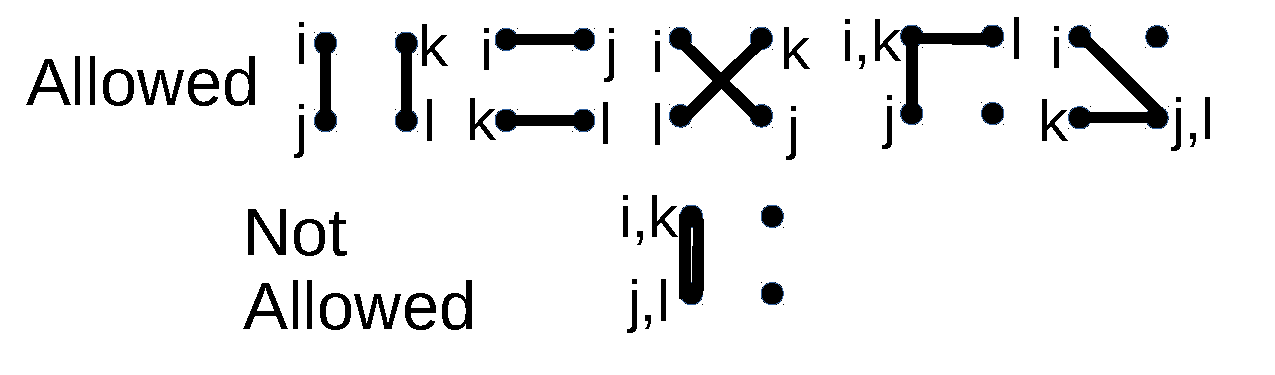
\includegraphics[width=1.0\textwidth]{../figures/pairing_fullquad.pdf}
\end{figure}
\end{frame}

\begin{frame}{Independent Pair Quadratic Correlations}
\begin{itemize}
   \item Or it can be expanded to get independent pair quadratic terms
   \begin{equation*}
   \begin{split}
      \ket{\psi_T} = \Bigg[\prod\limits_{i<j}&f_c(r_{ij})\Bigg] \Bigg[1+\fOpij \\
      & + \fOpij\fOqklip \Bigg] \ket{\phi}
   \end{split}
   \end{equation*}
\end{itemize}
\begin{figure}[h]
   \centering
   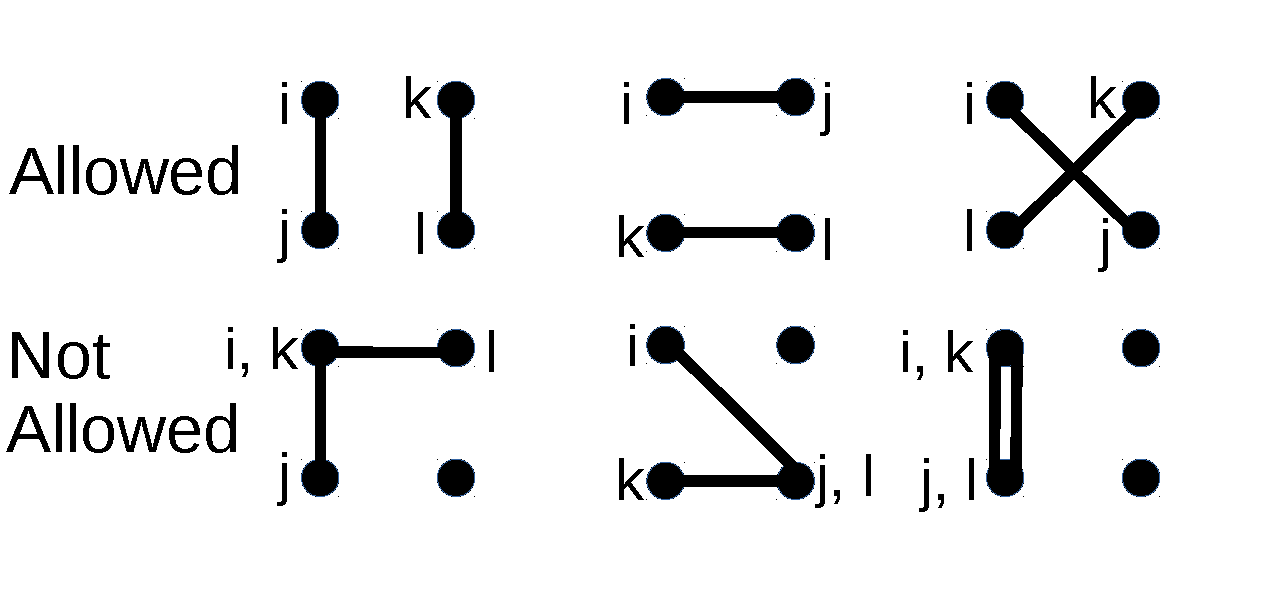
\includegraphics[width=0.7\textwidth]{../figures/pairing.pdf}
\end{figure}
\end{frame}

\begin{frame}{Results - AFDMC}
\begin{textblock*}{\textwidth}(0.0cm,-0.6cm) % {block width} (coords)
\begin{figure}[h]
   \centering
   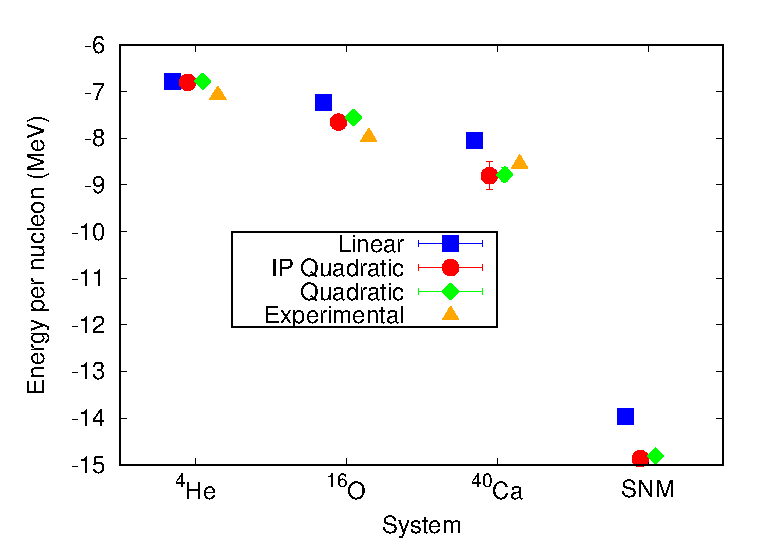
\includegraphics[width=0.6\textwidth]{../figures/energy.eps}
\end{figure}
\end{textblock*}
~\\~\\~\\~\\~\\~\\~\\~\\
\tiny
\begin{table}[htb]
\centering
\caption[]{Energy (*per nucleon) in MeV}
\begin{tabular}{ccccc}
\hline\hline
System & Linear & IP Quadratic & Quadratic & Experimental\\
\hline
%${}^{4}${He}   & -27.14(4) & -27.22(3)    & -27.11(3)    & -28.295   \\
%${}^{16}${O}   & -115.7(9) & -121.5(1.5)  & -120.0(1.4)  & -127.62   \\
%${}^{40}${Ca}  & -324(3)   & -347(8)      & -349(5)      & -342.1    \\
%SNM*           & -13.92(6) & -14.80(7)    & -14.70(11)   &           \\
${}^{4}${He}   & -27.14(4) & -27.19(3)    & -27.11(3)    & -28.296   \\
${}^{16}${O}   & -115.7(9) & -122.4(1.5)  & -120.8(1.3)  & -127.62   \\
${}^{40}${Ca}  & -322(3)   & -350(10)     & -351(6)      & -342.1    \\
SNM*           & -13.97(3) & -14.87(4)    & -14.81(3)    &           \\
\hline\hline
\end{tabular}
\label{tab:psi2}
\end{table}
{\tiny D. Lonardoni et al. \textit{Phys. Rev. C.,} \textbf{97}, 044318, 2018.}
\end{frame}
\note{
   \begin{itemize}
      \item Don't expect AV6' to reproduce experimental data
      \item 4He still doesn't change
      \item Decrease for larger systems, AND IP and full quad are the same.
   \end{itemize}
}

\begin{frame}{Results - VMC}
   \begin{figure}[h]
      \centering
      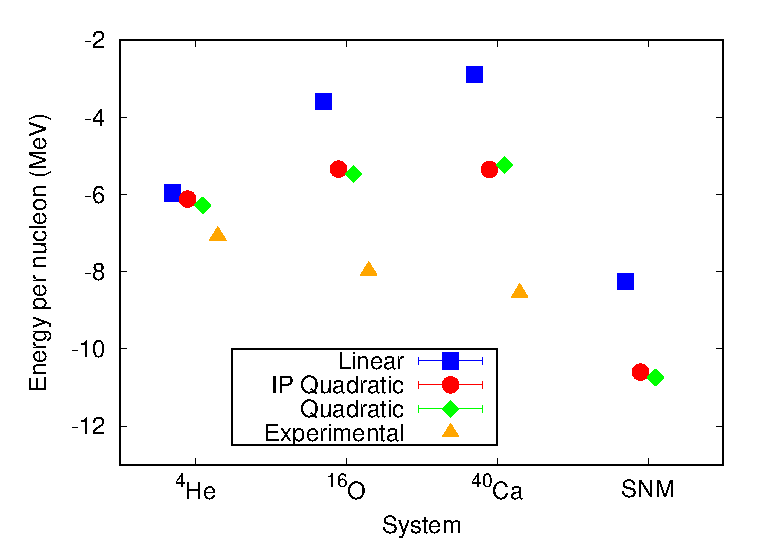
\includegraphics[width=0.8\textwidth]{../figures/energy_vmc.eps}
   \end{figure}
\end{frame}
\note{
   \begin{itemize}
      \item Sanity check since AFDMC doesn't have upper bound constraint like VMC.
      \item ALL decreased in energy, even 4He.
   \end{itemize}
}

\begin{frame}{Quadratic Correlation Cost}
\begin{figure}[h]
   \centering
   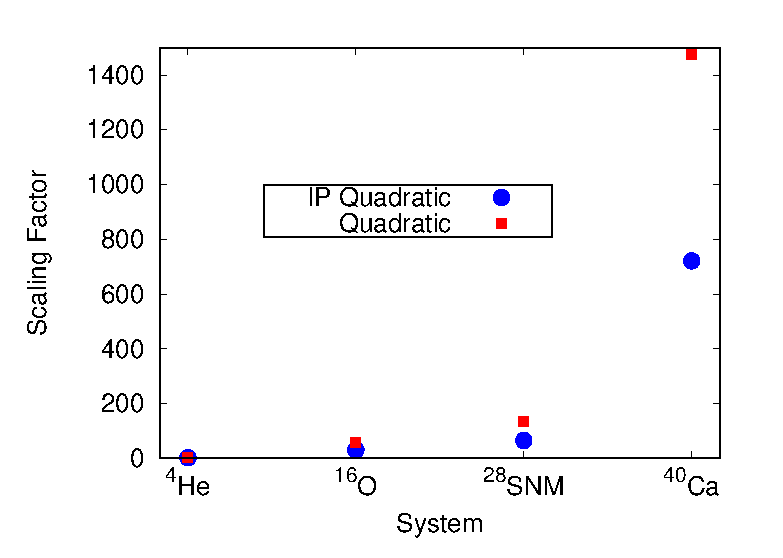
\includegraphics[width=0.65\textwidth]{../figures/scaling.eps}
\end{figure}
\vspace{-0.2cm}
\begin{table}[h!]
   \centering
   \begin{tabular}{ccccc}
      \hline \hline
       & $^{4}$He & $^{16}$O & SNM(28) & $^{40}$Ca \\
      \hline
      IP Quadratic & 1.73 & 30.7 & 64.8 & 720.9 \\
      Quadratic & 2.00 & 58.8 & 133.6 & 1473.9 \\
      \hline \hline
   \end{tabular}
\end{table}
\end{frame}

\begin{frame}{Results - $\chi$EFT up to N2LO - Preliminary}
\begin{table}[htb]
   \centering
   \begin{tabular}{llccc}
      \hline
      Calculation & Correlations & $^4$He & $^{16}$O & SNM \\
      \hline
      VMC   & Linear       & $-5.86(1)$ & $-1.08(1)$ & $1.56(5)$ \\
      VMC   & IP Quadratic & $-$        & $-4.03(4)$ & $-$ \\
      VMC   & Quadratic    & $-6.72(1)$ & $-3.95(4)$ & $-$ \\
      \hline
      AFDMC & Linear       & $-6.89(2)$ & $-5.74(4)$ & $-9.5(1)$ \\
      AFDMC & IP Quadratic & $-$        & $-7.3(2)$  & $-12.5(1)$ \\
      AFDMC & Quadratic    & $-6.91(2)$ & $-6.9(2)$  & $-12.6(1)$ \\
      \hline
   \end{tabular}
   \label{tab:chiquad}
\end{table}
\end{frame}
\note{
\begin{itemize}
   \item N2LO with $R_0 = 1$ fm cutoff.
   \item All the energies are per particle, in MeV.
   \item All the wave functions have both two- and three-body correlations.
   \item Local chiral potential at N2LO for R0=1.0fm cutoff.
   \item 4He and SNM are done with the E1 parametrization.
   \item 16O is done with the Etau parametrization.
   \item 4He and 16O also contain the Coulomb.
   \item Re-optimized for 4He and 16O with quadratic.
   \item No re-optimization for SNM and only used growth energy.
   \item SNM with no correction for finite size effects.
   \item All DMC with constrained-path, no transient/unconstrained.
\end{itemize}
}

\begin{frame}{Exponential Correlations}
\begin{equation*}
   \ket{\psi_T} = \left[\prod\limits_{i<j}f_c(r_{ij})\right] e^{\sum\limits_{i<j}\sum\limits_p\fpij\Opij} \ket{\phi}
\end{equation*}
\begin{itemize}
   \item This looks just like the propagator and so we can {\bf use the same trick} with the HS transformation.
\begin{align*}
   G_{SD}(R'S',RS,\dt) &= \bra {R'S'}e^{-\sum\limits_{p=2}^6\sum\limits_{i<j}v_p(r_{ij})\Opij\dt} \ket{RS} \\
      &= \prod\limits_{n=1}^{15A}\frac{1}{\sqrt{2\pi}}\int dx_n e^{-\frac{x_n^2}{2}}e^{\sqrt{-\lambda_n\dt} x_nO_n}
\end{align*}
\end{itemize}
\end{frame}

\begin{frame}{Exponential Correlations}
\begin{itemize}
   \item 
\end{itemize}
\begin{equation*}
   \exp\left(\sum\limits_{i<j,p}f_p(r_{ij})\Opij\right) = \prod\limits_{n=1}^{15A} \frac{1}{\sqrt{2\pi}}\int dx_n e^{-x_n^2/2}e^{\sqrt{\lambda_n}x_nO_n}.
\end{equation*}
\end{frame}

\subsection{Alpha Formation in NS}
\begin{frame}{Placeholder}
blah
\end{frame}

\section{Conclusion}
\subsection{Conclusion}
\begin{frame}{Placeholder}
blah
\end{frame}
\subsection{Future Work}

\appendix
\begin{frame}{Extra Slides}
\begin{centering}
   Extra Slides
\end{centering}
\end{frame}

\begin{frame}{$\chi$EFT vs. AV6$'$}
\red{Slide comparing the AV6$'$ results with N2LO results. Remember that N2LO has the spin-orbit, which decreases binding.}
\end{frame}

%\note[itemize]{
%   \item test1
%   \item test2
%}

\end{document}
